\section[Requisitos e Rastreabilidade]{Requisitos e Rastreabilidade}
A rastreabilidade pode ser definida como a habilidade de se acompanhar a vida
de um requisito em ambas as direções do processo de software e durante todo o ciclo de
vida. Ela fornece uma base para o desenvolvimento de uma trilha de auditoria para todo
o projeto, possibilitando encontrar outros requisitos e artefatos que podem ser afetados
pelas mudanças solicitadas (PALMER, 1997). 

Para tal, é necessário haver ligações entre requisitos e entre requisitos e outros elementos do processo de software. Assim, a identificação da composição de requisitos, das dependências entre requisitos, de
requisitos conflitantes, da origem dos requisitos e de seus interessados, além da
identificação de em quais artefatos produzidos durante o desenvolvimento de software
um requisito é tratado, é de fundamental importância para que a rastreabilidade possa
ser implementada (WIEGERS, 2003; ROBERTSON; ROBERTSON, 2006;
KOTONYA; SOMMERVILLE, 1998). 

A rastreabilidade se encaixa em nosso projeto de maneira bidirecional, onde é
possível rastrear a dependência entre os todos os níveis de abstração do projeto,
épicos, features e histórias de usuário.

Esse tipo de rastreabilidade deve tanto acontecer na forma horizontal quanto
na vertical. A rastreabilidade bidirecional é importante para analisar o impacto
de mudanças (em direção à implementação) e verificar a satisfação dos
requisitos (em direção à origem).

A imagem abaixo é a matriz de rastreabilidade do nosso projeto que foi gerada pela ferramente TargetProcess. Nela podem ser identificadas os épicos, features e histórias de usuário.

\begin{figure}[!htb]
    \centering
    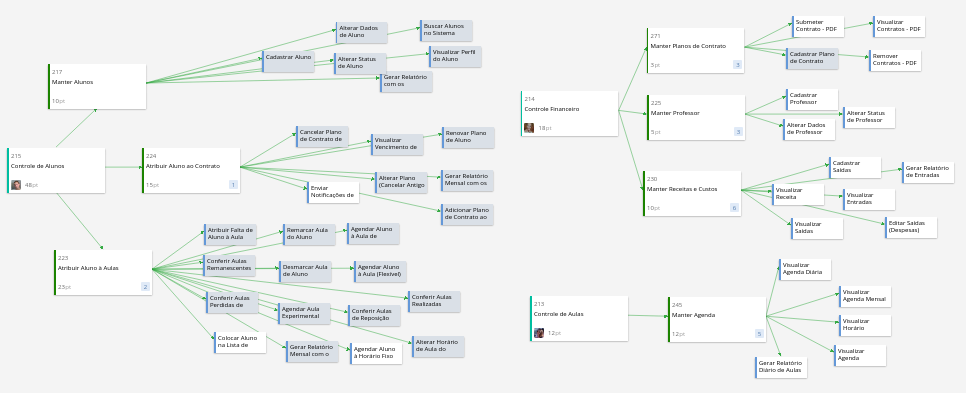
\includegraphics[width=1.5\textwidth, angle=-90]{figuras/matriz_rastreabilidade.png}
    \caption{Matriz de Rastreabilidade}
    \label{fig:matriz_rastreabilidade}
\end{figure}
